\section{Relasjoner}
\subsection{Relasjoner}
\begin{frame}[fragile]{Relasjoner}
    En relasjon $R$ fra $A$ til $B$ er et subset $ R \subseteq A \times B$. De minner om funksjoner, men er et mer generelt konsept. De er lettere å visualisere ved å tegne dem:
    \begin{figure}
        \centering
        \subfloat{{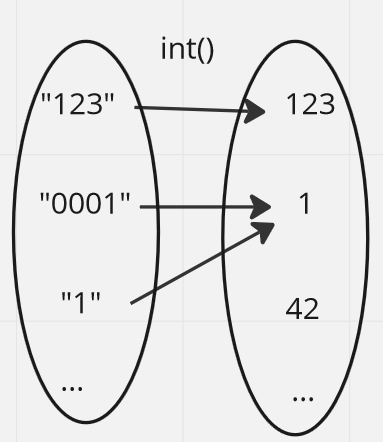
\includegraphics[width=2.8cm]{images/int again.png} }}
        \qquad
        \subfloat{{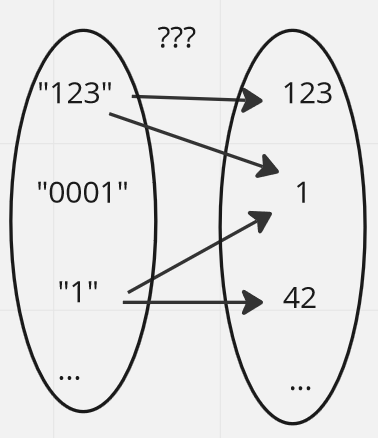
\includegraphics[width=2.8cm]{images/???.png} }}
        \qquad
        \subfloat{{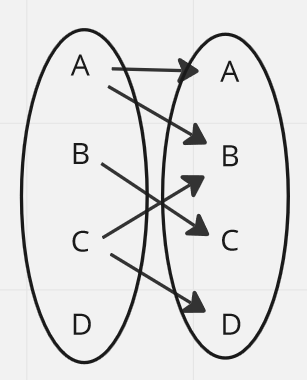
\includegraphics[width=2.8cm]{images/aa.png} }}
        \qquad
        \subfloat{{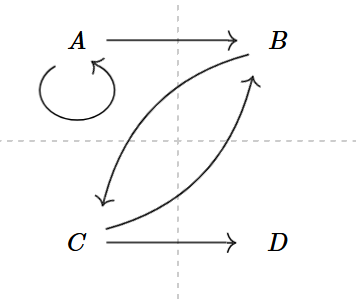
\includegraphics[width=2.8cm]{images/aaa.png} }}
        \label{fig:relasjoner}
    \end{figure} 

    \pause
    Veldig ofte er $A$ og $B$ det samme settet, dvs at $R \subseteq A \times A$.\\ 
    Da kaller vi R en relasjon \emph{på} $A$.
\end{frame}

\begin{frame}[fragile]{Måter å oppgi relasjoner på}
    \begin{columns}
        \begin{column}{0.3\textwidth}
            \begin{tikzcd}
            A \arrow[r] \arrow[d] \arrow[rd] & B \arrow[d] \arrow[ld] \\
            D                                & C \arrow[l]           
            \end{tikzcd}
        \end{column}
        \begin{column}{0.65\textwidth}
            \pause
            Kantliste:\\
            $\{(A, B), (A, C), (A, D), (B, C), (B, D), (C, D)\}$\\[5mm]
            \pause
            Settkomprehensjon:\\
            $\{(x, y) | x, y \in \{A,B,C,D\}, x < y\}$:\\[5mm]
            \pause
            \begin{columns}
                \begin{column}{0.27\textwidth}
                    Matrise:\\
                    \begin{math}
                        \begin{matrix}
                              & A & B & C & D\\
                            A & 0 & 1 & 1 & 1\\
                            B & 0 & 0 & 1 & 1\\
                            C & 0 & 0 & 0 & 1\\
                            D & 0 & 0 & 0 & 0
                        \end{matrix}
                    \end{math}
                \end{column}
                \pause
                \begin{column}{0.38\textwidth}
                    Nabolister:\\        
                    $N(A) = [B, C, D]$\\
                    $N(B) = [C, D]$\\
                    $N(C) = [D]$\\
                    $N(D) = []$
                \end{column} 
            \end{columns}
        \end{column}
    \end{columns}
\end{frame}

\subsection{Egenskaper}
\begin{frame}[fragile]{Egenskaper på relasjoner}
Gitt en relasjon $R \subseteq A \times A$ på $A$ har vi 5 viktige begreper for å beskrive den:
    \begin{itemize}
        \item Refleksiv: $\forall a : ((a, a) \in R)$
        \pause
        \item Symmetrisk: $\forall a, b : [(a, b) \in R \leftrightarrow (b, a) \in R]$
        \pause
        \item Antisymmetrisk: $\forall a, b : [(a, b) \in R \land (b, a) \in R \rightarrow a = b]$
        \pause
        \item Transitiv: $\forall a, b, c : [(a, b) \in R \land (b, c) \in R \rightarrow (a, c) \in R]$\\
        \pause
        \item Om en relasjon er refleksiv, symmetrisk og transitiv, kaller vi det en ekvivalensrelasjon.
    \end{itemize}   
\end{frame}

\begin{frame}[fragile]{Refleksive relasjoner}
En relasjon $R$ er \emph{refleksiv} hvis $\forall a : ((a, a) \in R)$.\\
    \begin{columns}
        \begin{column}{0.3\textwidth}
        Ikke refleksiv:\\
        \adjustbox{scale=0.8}{
            \begin{tikzcd}
            a \arrow[dd] \arrow[rr] &  & b                                             \\
                                    &  &                                               \\
            c \arrow[rruu]          &  & d \arrow[loop, distance=2em, in=305, out=235]
            \end{tikzcd}
        }  
        \end{column}
        \pause
        \begin{column}{0.3\textwidth}
            Refleksiv:\\
            \adjustbox{scale=0.8}{
                \begin{tikzcd}
                a \arrow[dd] \arrow[rr] \arrow[loop, distance=2em, in=305, out=235] &  & b \arrow[loop, distance=2em, in=305, out=235] \\
                                                                                    &  &                                               \\
                c \arrow[rruu] \arrow[loop, distance=2em, in=305, out=235]          &  & d \arrow[loop, distance=2em, in=305, out=235]
                \end{tikzcd}
            }
        \end{column}
    \end{columns}
    \pause
    \begin{columns}
        \begin{column}{0.3\textwidth}
            \begin{math}
                \begin{matrix}
                      & a & b & c & d\\
                    a & 0 & 1 & 1 & 0\\
                    b & 0 & 0 & 0 & 0\\
                    c & 0 & 1 & 0 & 0\\
                    d & 0 & 0 & 0 & 1
                \end{matrix}
            \end{math}
        \end{column}
        \begin{column}{0.3\textwidth}
            \begin{math}
                \begin{matrix}
                      & a & b & c & d\\
                    a & 1 & 1 & 1 & 0\\
                    b & 0 & 1 & 0 & 0\\
                    c & 0 & 1 & 1 & 0\\
                    d & 0 & 0 & 0 & 1
                \end{matrix}
            \end{math}
        \end{column}
    \end{columns}
\end{frame}

\begin{frame}[fragile]{Symmetriske relasjoner}
    En relasjon $R$ er \emph{symmetrisk} hvis $\forall a, b : [(a, b) \in R \leftrightarrow (b, a) \in R]$.\\
    \begin{columns}
        \begin{column}{0.3\textwidth}
            Ikke symmetrisk:\\
            \adjustbox{scale=0.8}{
                \begin{tikzcd}
                    a \arrow[dd]   &  & b                                             \\
                                   &  &                                               \\
                    c \arrow[rruu] &  & d \arrow[loop, distance=2em, in=305, out=235]
                \end{tikzcd}
            }
        \end{column}
        \pause
        \begin{column}{0.3\textwidth}
            Symmetrisk:\\
            \adjustbox{scale=0.8}{
                \begin{tikzcd}
                    a \arrow[dd, bend left]                          &  & b \arrow[lldd, bend right]                    \\
                                                                     &  &                                               \\
                    c \arrow[rruu, bend right] \arrow[uu, bend left] &  & d \arrow[loop, distance=2em, in=305, out=235]
                \end{tikzcd}
            }
        \end{column}
    \end{columns}
    \pause
    \begin{columns}
        \begin{column}{0.3\textwidth}
            \begin{math}
                \begin{matrix}
                      & a & b & c & d\\
                    a & 0 & 0 & 1 & 0\\
                    b & 0 & 0 & 0 & 0\\
                    c & 0 & 1 & 0 & 0\\
                    d & 0 & 0 & 0 & 1
                \end{matrix}
            \end{math}
        \end{column}
        \begin{column}{0.3\textwidth}
            \begin{math}
                \begin{matrix}
                      & a & b & c & d\\
                    a & 0 & 0 & 1 & 0\\
                    b & 0 & 0 & 1 & 0\\
                    c & 1 & 1 & 0 & 0\\
                    d & 0 & 0 & 0 & 1
                \end{matrix}
            \end{math}
        \end{column}
    \end{columns}
\end{frame}

\begin{frame}[fragile]{Antisymmetriske relasjoner}
    En relasjon $R$ er \emph{antisymmetrisk} hvis $\forall a, b : [(a, b) \in R \land (b, a) \in R \rightarrow a = b]$.\\
    \begin{columns}
        \begin{column}{0.3\textwidth}
            Ikke antisymmetrisk:\\
            \adjustbox{scale=0.8}{
                \begin{tikzcd}
                a \arrow[dd, bend left]                          &  & b \arrow[lldd, bend right]                    \\
                                                                 &  &                                               \\
                c \arrow[rruu, bend right] \arrow[uu, bend left] &  & d \arrow[loop, distance=2em, in=305, out=235]
                \end{tikzcd}
            }
        \end{column}
        \pause
        \begin{column}{0.3\textwidth}
            Antisymmetrisk:\\
            \adjustbox{scale=0.8}{
                \adjustbox{scale=0.8}{
                    \begin{tikzcd}
                        a \arrow[dd]   &  & b                                             \\
                                       &  &                                               \\
                        c \arrow[rruu] &  & d \arrow[loop, distance=2em, in=305, out=235]
                    \end{tikzcd}
                }
            }
        \end{column}
    \end{columns}
    \pause
    \begin{columns}
        \begin{column}{0.3\textwidth}
            \begin{math}
                \begin{matrix}
                      & a & b & c & d\\
                    a & 0 & 0 & 1 & 0\\
                    b & 0 & 0 & 1 & 0\\
                    c & 1 & 1 & 0 & 0\\
                    d & 0 & 0 & 0 & 1
                \end{matrix}
            \end{math}
        \end{column}
        \begin{column}{0.3\textwidth}
            \begin{math}
                \begin{matrix}
                      & a & b & c & d\\
                    a & 0 & 0 & 1 & 0\\
                    b & 0 & 0 & 0 & 0\\
                    c & 0 & 1 & 0 & 0\\
                    d & 0 & 0 & 0 & 1
                \end{matrix}
            \end{math}
        \end{column}
    \end{columns}
\end{frame}

\begin{frame}[fragile]{Transitive relasjoner}
    En relasjon $R$ er \emph{transitiv} om $\forall a, b, c : [(a, b) \in R \land (b, c) \in R \rightarrow (a, c) \in R]$.\\
    \begin{columns}
        \begin{column}{0.3\textwidth}
            Ikke transitiv:
             \begin{tikzcd}
            a \arrow[r] \arrow[d] & b \arrow[d] \\
            d                     & c          
            \end{tikzcd}
        \end{column}
        \pause
        \begin{column}{0.3\textwidth}
            Transitiv:
            \begin{tikzcd}
            a \arrow[r] \arrow[d] \arrow[rd] & b \arrow[d] \\
            d                                & c          
            \end{tikzcd}
        \end{column}
    \end{columns}
\end{frame}

\begin{frame}{Relasjonskomposisjon}
    Gitt to relasjoner $R \subseteq A \times B$ og $S \subseteq B \times C$, kan vi konstruere komposisjonen $S \circ R \subseteq A \times C$:\\
    $S \circ R := \{(a, c) | (a, b) \in R \land (b, c) \in S\}$
    \pause
    \begin{figure}%
        \centering
        \subfloat{{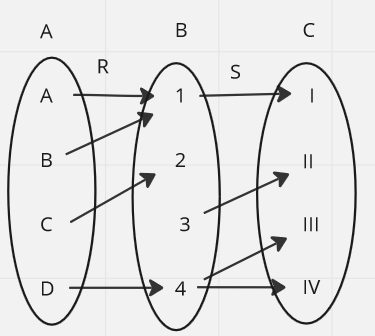
\includegraphics[width=3.3cm]{images/R, S.png} }}%
        \qquad
        \subfloat{{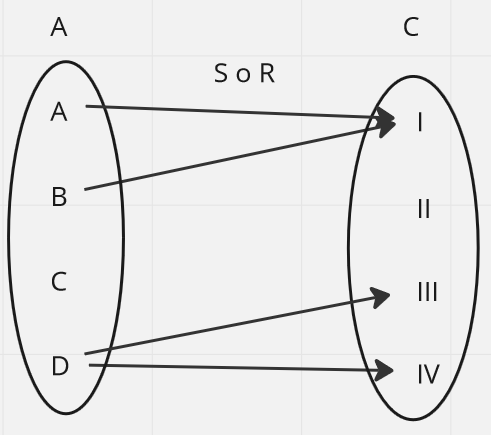
\includegraphics[width=3.3cm]{images/S o R.png} }}%
        \label{fig:ros}%
    \end{figure}
    \pause
    Obs! Som med funksjonskomposisjon er rekkefølgen er uintuitiv: R skjer før S. Dere kan lese det som $S$ 'på' $R$.
\end{frame}

\begin{frame}{Tavleoppgaver om relasjoner}
    Avgjør om følgende relasjoner er refleksive, symmetriske, anti-symmetriske, eller transitive. Er noen av dem ekvivalenserelasjoner?\\
    \begin{center}
    \begin{tabular}{ | m{15em} | m{1cm} | m{1cm} | m{1.5cm} | m{1cm} | m{1cm} | } 
      \hline
      Relasjon & Refl. & Symm. & A. Symm. & Trans. & Ekv.\\
      \hline
      $\{(a, b) | a, b \in \mathbb{N}, a < b\}$ \pause & \xmark & \xmark & \checkmark & \checkmark & \xmark \\
      \hline
      \pause
      $\{(a, b) | a, b \in \mathbb{N}, a \leq b\}$ \pause & \checkmark & \xmark & \checkmark & \checkmark & \xmark \\
      \hline
      \pause
      $B_{p, q}$ := Alle logiske uttrykk gitt av $p$ og $q$; $\{(a, b) | a, b \in B_{p, q}, a \equiv b\}$ \pause & \checkmark & \checkmark & \xmark & \checkmark & \checkmark\\
      \hline
      \pause
      $\emptyset$ \pause & \checkmark & \checkmark & \checkmark & \checkmark & \checkmark\\
      \hline
    \end{tabular}
    \end{center}
    \pause
    Merk at symmetri og antisymmetri ikke er helt det motsatte. En relasjon kan være begge deler (som $\emptyset$), og en relasjon kan være ingen av dem.
\end{frame}

\subsection*{Spørretid}
\begin{frame}{Spørsmål?}
    \begin{figure}
        \centering
        
\includegraphics[height = 4.9cm]{images/guillaume3.jpg}
        \caption{Guillaume et sted Lukas ikke husker}
        \label{fig:guillaume3}
    \end{figure}
\end{frame}